%; whizzy chapter
% -initex iniptex -latex platex -format platex -bibtex jbibtex -fmt fmt
% 以上 whizzytex を使用する場合の設定。

%     Kansai Debian Meeting resources
%     Copyright (C) 2007 Takaya Yamashita
%     Thank you for Tokyo Debian Meeting resources

%     This program is free software; you can redistribute it and/or modify
%     it under the terms of the GNU General Public License as published by
%     the Free Software Foundation; either version 2 of the License, or
%     (at your option) any later version.

%     This program is distributed in the hope that it will be useful,
%     but WITHOUT ANY WARRANTY; without even the implied warranty of
%     MERCHANTABILITY or FITNESS FOR A PARTICULAR PURPOSE.  See the
%     GNU General Public License for more details.

%     You should have received a copy of the GNU General Public License
%     along with this program; if not, write to the Free Software
%     Foundation, Inc., 51 Franklin St, Fifth Floor, Boston, MA  02110-1301 USA

%  preview (shell-command (concat "evince " (replace-regexp-in-string "tex$" "pdf"(buffer-file-name)) "&"))
% 画像ファイルを処理するためにはebbを利用してboundingboxを作成。
%(shell-command "cd image200708; ebb *.png")

%%ここからヘッダ開始。

\documentclass[mingoth,a4paper]{jsarticle}
\usepackage{kansaimonthlyreport}
\usepackage[dvips]{xy}
\usepackage{ulem}

% 日付を定義する、毎月変わります。
\newcommand{\debmtgyear}{2013}
\newcommand{\debmtgdate}{27}
\newcommand{\debmtgmonth}{10}
\newcommand{\debmtgnumber}{77}

\def\fixme#1{{\color{red}{#1}}}

\begin{document}

\begin{titlepage}

% 毎月変更する部分、本文の末尾も修正することをわすれずに

 第\debmtgnumber{}回 関西 Debian 勉強会資料

\vspace{2cm}

\begin{center}
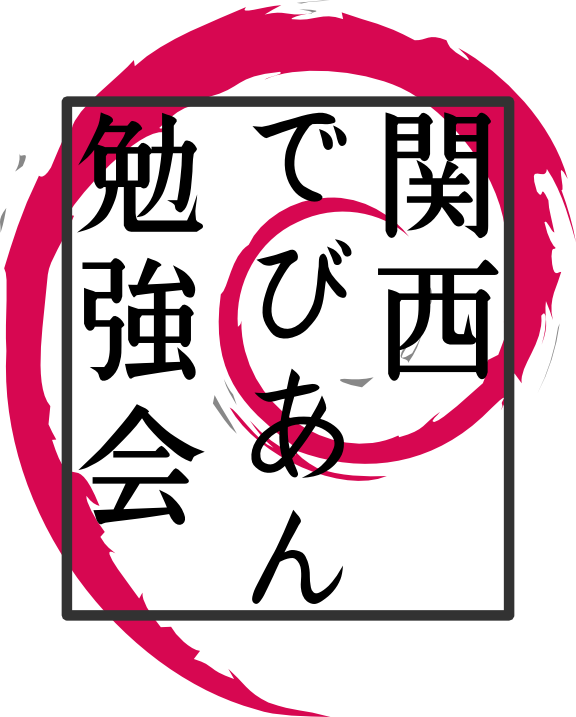
\includegraphics{image200802/kansaidebianlogo.png}
\end{center}

\begin{flushright}
\hfill{}関西 Debian 勉強会担当者 佐々木・倉敷・のがた・かわだ・八津尾 \\
\hfill{}\debmtgyear{}年\debmtgmonth{}月\debmtgdate{}日
\end{flushright}

\thispagestyle{empty}
\end{titlepage}

\dancersection{Introduction}{Debian JP}

\vspace{1em}

 関西Debian勉強会はDebian GNU/Linuxのさまざまなトピック
 (新しいパッケージ、Debian特有の機能の仕組、Debian界隈で起こった出来事、
 などなど)について話し合う会です。

 目的として次の三つを考えています。
 \begin{itemize}
  \item MLや掲示板ではなく、直接顔を合わせる事での情報交換の促進
  \item 定期的に集まれる場所
  \item 資料の作成
 \end{itemize}

 それでは、楽しい一時をお過ごしください。

\newpage

\begin{minipage}[b]{0.2\hsize}
 {\rotatebox{90}{\fontsize{80}{80}
{\gt 関西 Debian 勉強会}}}
\end{minipage}
\begin{minipage}[b]{0.8\hsize}
\hrule
\vspace{2mm}
\hrule
\setcounter{tocdepth}{1}
\tableofcontents
\vspace{2mm}
\hrule
\end{minipage}

\dancersection{最近のDebian関係のイベント報告}{Debian JP}

\subsection{第 76 回関西 Debian 勉強会}

76 回目の関西 Debian 勉強会は 9 月 22 日(日)に、港区民センターで行なわ
れました。

セッションは坂本さんによる「Linuxとサウンドシステム」と倉敷さんによる
「dgit でソースパッケージを触ってみる」の二本でした。

dgit はまだ DD しか使うことのできないツールで、どうなることかと思われ
ましたが、飛び込みで DD が来られて実演することができました。アップスト
リームが git で、パッケージを git で管理するには便利そうなツールですね。

Linux のサウンドシステムは時間切れで途中で終わってしまいましたので、今
回、後半の続きとなります。

\subsection{第 105 回東京エリア Debian 勉強会}

105 回目の東京エリア Debian 勉強会は 10 月 20 日(日)に OSC 2013
Tokyo/Fall で出張開催されました。

初の日曜開催と天候のため例年より来場者が少かったようですが、ブース展示
は好評だったようです。

セッションは「Debian 最近の update」として Debian の最新情報について紹
介されました。中でも Debian カンファレンスの紹介は、ビデオ視聴での字幕
の設定の仕方や、おもしろいライトニングトークが紹介されていますので、是
非目を通してみてください。
\footnote{発表資料 \url{http://tokyodebian.alioth.debian.org/pdf/debianmeetingresume201310-presentation.pdf}}

\subsection{Debian Project}

\subsubsection{Bits from the Release Team (Jessie freeze info)}

Jessie のフリーズ日が 2014/11/5 23:59(UTC) とアナウンスされました。
\footnote{\url{http://lists.debian.org/debian-devel-announce/2013/10/msg00004.html}}

Wheezy のフリーズ日が 2012/6/30 でしたので 2 年毎のフリーズなら 2014/6
の終わりごろになるのですが、2 年毎のリリース、半年のフリーズ期間を優先
して 2014/11/5 となったようです。5 日というのは、"Gunpowder day"
\footnote{\url{https://en.wikipedia.org/wiki/Gunpowder_plot}}
\footnote{\url{https://en.wikipedia.org/wiki/Guy_Fawkes_Night}}
だから覚えやすいでしょということらしいです。

\newpage

また、リリースゴールに次の提案があり、検討中となっています。

\begin{screen}
  \begin{itemize}
  \item Native systemd support in every package with sysv scripts
  \item Hardening of ELF binaries (carry over from Wheezy)
  \item debian/rules to honor CC/CXX flags
  \item clang as secondary compiler
  \item piuparts clean archive
  \item Cross Toolchains in the archive
  \item Make the base system cross-buildable
  \item SELinux
  \item UTF-8
  \end{itemize}
\end{screen}

\subsubsection{debian-devel@d.o}

「systemd effectively mandatory now due to GNOME」
\footnote{\url{http://lists.debian.org/debian-devel/2013/10/msg00444.html}}
から始まって、
「Proposal: switch default desktop to xfce」
\footnote{\url{http://lists.debian.org/debian-devel/2013/10/msg00496.html}}
に続き、
「Proposal: switch init system to systemd or upstart」
\footnote{\url{http://lists.debian.org/debian-devel/2013/10/msg00651.html}}
へと、恒例の話題で盛り上ってます。
ここ 2、3 日で 200 通ほどのメールが流れているので興味のある方は追ってみてください。


\dancersection{事前課題}{Debian JP}

今回の課題は以下の通りです。
\begin{screen}
  \begin{enumerate}
  \item %
    パッケージlibasound2-devをインストールし、
    添付の pcm\_minimal.c をコンパイルして実行ファイルを作成してください。
    実行ファイルを実行した結果を教えてください。
  \item %
    git-buildpackage を install してきて下さい。
  \item %
    Debian Developer/Maintainer の方は, 御自身がメンテされているパッケージをどの VCS で管理されているかお答え下さい。
    パッケージをメンテされていない方は、
    \begin{center}
      {\tt{http://anonscm.debian.org/gitweb}}
    \end{center}
    以下にあるパッケージを眺めて触ってみたいパッケージを決めておいて下さい。
  \end{enumerate}
\end{screen}

参加者の皆さんの解答は以下の通りです:

\begin{prework}{ 坂本 貴史 }
  \begin{enumerate}
  \item ノイズが聞こえました
  \item インストールできました
  \item debootstrapをやりたいと思います
  \end{enumerate}
\end{prework}

\begin{prework}{ kozo2 }
  \begin{enumerate}
  \item まだやっています。とりいそぎ参加申し込みしておきたいので結果は会場で口頭で述べさせてください。
  \item いまinstallしようとしています
  \item メンテしていないです。pkg-ruby-extras/ruby-bio.git, pkg-mozext/firebug.git, aptitude/aptitude.git を触ってみたいです
  \end{enumerate}
\end{prework}

\begin{prework}{ lurdan }
  \begin{enumerate}
  \item あとでやっておきます。
  \item essential ですよ?
  \item git
  \end{enumerate}
\end{prework}

\begin{prework}{ 西原 }
  \begin{enumerate}
  \item noisyでした。
  \item installしました。
  \item 触ってみたいパッケージを決めておきます。
  \end{enumerate}
\end{prework}

\begin{prework}{ 西山和広 }
  \begin{enumerate}
  \item ザーというアナログテレビの砂嵐のような音が出ました。
  \item インストールしました。
  \item twitter irc gateway の atig が普段使っているので良さそうだと思いました。
  \end{enumerate}
\end{prework}

\begin{prework}{ おくの }
  \begin{enumerate}
  \item ノイズ音が鳴りました。
  \item インストールしました。
  \item OpenStackパッケージとか個人的に興味ありますが多いですねー
  \end{enumerate}
\end{prework}

\begin{prework}{ 川江 }
  \begin{enumerate}
  \item コンパイルに失敗しました。
  \item しました
  \item qemu-kvm
  \end{enumerate}
\end{prework}

\begin{prework}{ かわだてつたろう }
  \begin{enumerate}
  \item なにもおこりませんでした。

    ソースをみるとノイズ音がするのでしょうか。
  \item はい。
  \item メンテしていないので、何か決めておきます。
  \end{enumerate}
\end{prework}

\begin{prework}{ 佐々木洋平 }
  \begin{enumerate}
  \item はい。

    \begin{commandline}
% gcc -Wall -Wextra -c pcm_minimal.c
pcm_minimal.c: 関数 ‘main’ 内:
pcm_minimal.c:48:4: 警告: ‘if’ 文内の空の本体は中括弧で括ることを推奨します [-Wempty-body]
    ; /* cannot resolve XRUN */
    ^
pcm_minimal.c:50:4: 警告: ‘if’ 文内の空の本体は中括弧で括ることを推奨します [-Wempty-body]
    ; /* cannot write all of samples */
    ^
pcm_minimal.c:19:6: 警告: 使用されない変数 ‘err’ です [-Wunused-variable]
  int err;
% gcc -Wall -Wextra -o pcm_minimal pcm_minimal.o -lasound
    \end{commandline}
  \item はい. 
  \item 自分の関与しているパッケージは pkg-ruby-extras に沢山あったりします。
  \end{enumerate}
\end{prework}

\begin{prework}{ 大林 }
  \begin{enumerate}
  \item コンパイルしました。実行するとヘッドフォンからノイズ音が出力されます。
  \item しました
  \item メンテナではないので何か考えておきます。

    mesa とか yard とか?
  \end{enumerate}
\end{prework}

\begin{prework}{ yabuki@netfort.gr.jp }
  \begin{enumerate}
  \item Nothing happened
  \item はい、やっときました。
  \item むかし、yc-el を svn-buildpackage でやっていたが、これぼめんてがなくなったので、もうありません。
  \end{enumerate}
\end{prework}

\dancersection{ALSAのユーザーランド解説}{坂本 貴史}

\begin{itemize}
\item ライブラリ、設定ファイル、プラグインなどがある
\item ドキュメントはパッケージ「{\tt libasound2-doc}」で「{\tt /usr/share/doc/libaound2-doc/html/}」以下へインストールできる
\item Androidは独自にユーザーランドの実装を持っている
\end{itemize}

\subsection{ライブラリ}
\begin{itemize}
\item  asound
\item 設定ファイルのパース機能を持つ
  \begin{itemize}
  \item  システムレベル、ユーザーレベルでランタイム設定
  \end{itemize}
\item プラグインを持つ
  \begin{itemize}
  \item 任意の機能を付与できる
  \end{itemize}
\end{itemize}

\subsection{PCMノード}
\begin{itemize}
\item ランタイムに設けられる。
\item {\tt aplay -L}あるいは{\tt arecord -L}で一覧を取得できる。
\item PCMのキャラクターデバイスを隠蔽し特定の機能を付与したもの
\item この特定の機能を付与するために用いられるのがPCMプラグイン
\item 設定ファイルがPCMノードを設けている
\item ライブラリのPCMインターフェイスでハンドルを開く時に指定する
\end{itemize}

\begin{commandline}
$ aplay -L
default
    Playback/recording through the PulseAudio sound server
sysdefault:CARD=Intel
    HDA Intel, ALC889 Analog
    Default Audio Device
front:CARD=Intel,DEV=0
    HDA Intel, ALC889 Analog
    Front speakers
surround40:CARD=Intel,DEV=0
    HDA Intel, ALC889 Analog
    4.0 Surround output to Front and Rear speakers
surround41:CARD=Intel,DEV=0
    HDA Intel, ALC889 Analog
    4.1 Surround output to Front, Rear and Subwoofer speakers
surround50:CARD=Intel,DEV=0
    HDA Intel, ALC889 Analog
    5.0 Surround output to Front, Center and Rear speakers
surround51:CARD=Intel,DEV=0
    HDA Intel, ALC889 Analog
    5.1 Surround output to Front, Center, Rear and Subwoofer speakers
surround71:CARD=Intel,DEV=0
    HDA Intel, ALC889 Analog
    7.1 Surround output to Front, Center, Side, Rear and Woofer speakers
\end{commandline}

\subsection{設定ファイル}
\begin{itemize}
\item ALSA特有の記法で書かれている
\item システムレベルは{\tt /usr/share/alsa}以下にある
  \begin{itemize}
  \item {\tt /usr/share/alsa/alsa.conf}の「{\tt defaults.namehint.extended off}」が、{\tt hw/plughw/dmix/dsnoop}の表示を抑制
  \end{itemize}
\item ユーザーレベルは「{\tt .asoundrc}」をホームディレクトリに配置
\end{itemize}

\subsection{プラグイン}
\begin{itemize}
\item プラグインには2つのタイプがある
  \begin{itemize}
  \item[PCMタイプ] PCMノードに機能を追加する
  \item[MIXERタイプ] Controlノードに機能を追加する
  \end{itemize}
\item {\tt aplay -L}でいろんなノードが見えるのはPCMプラグインのおかげ。
  \begin{itemize}
  \item[front] フロント出力のためのもの
  \item[surroundXXX] サラウンド出力のためのもの
  \item[hw] 標本化周波数、量子化ビット数、チャンネル数などをちゃんと指定する必要がある
  \item[plughw] 上記をよしなに設定してくれる
  \item[pulse] 出力をPulseAudioに流しこんだり、入力をPulseAudioから受けたりする
  \item[dmix] 複数の出力をひとつのストリームに合成する
  \item[dsnoop] ひとつの入力を複数のストリームにする
  \item[default] ALSAの配布するパッケージでは、dmix/dsnoopを入出力スレーブとしている
  \end{itemize}
\item その他のプラグイン
  \begin{itemize}
  \item[bluetooth] Bluezを利用して音声機能を持つBluetoothデバイスを使う
  \item[ladspa] LADSPAというフレームワークのプラグインを使う
  \end{itemize}
\end{itemize}

\subsection{PulseAudio}
\begin{itemize}
\item 複数のアプリケーションの出力を束ねたり、入力を分割したりする
\item 最近のデスクトップ環境は、libasound2のpulseプラグインを有効にし、defaultノードをpulseノードに設定

  こうすることで、ALSAを直接利用するアプリケーションの入出力をPulseAudioに向けている
\item PulseAudioのモジュール構造
  \begin{itemize}
  \item いろんな機能を共有ライブラリの形で提供。自在にロード・アンロードできる。
  \item \url{http://www.freedesktop.org/wiki/Software/PulseAudio/Documentation/User/Modules/}
  \end{itemize}
\item ALSA以外のサブシステムを使える
  \begin{itemize}
  \item Bluez
  \item Network
  \end{itemize}
\end{itemize}

\dancersection{git-buildpackage入門again}{佐々木 洋平}

\subsection{はじめに}

最近ではDebianパッケージの管理になんらかのバージョン管理システム(VCS)を使うことが一般的になってきました。
%
VCS usage for Debian source packages\footnote{%
  \label{footnote:1}
  (declared) VCS usage for Debian source packages:
  \texttt{http://upsilon.cc/\~{}zack/stuff/vcs-usage/}%
}によれば、
現状ではソースパッケージの $70.44\%$ がなんらかの VCS を使用しており、
そのうち $65\%$ が Git を使用しています\footnote{%
  上記URL$^{\ref{footnote:1}}$ によれば Subversion の利用が $28\%$、
  Git と subversion で全体の $93\%$ を占めています。
  近年、Subversion から Git へ移行するチームが増えていることもあり、
  先月の dgit 含め、
  今後は Git による Debian パッケージの管理が主流となるのかもしれません。
}。
そんな訳で、Git によるパッケージ管理の知識はそろそろマストアイテムになりつつあるのかもしれません。

Debian パッケージを Git で管理するために使われるソフトウェアとして代表的なのが
\texttt{git-buildpackage} です。
これまでにも勉強会において
\texttt{git-buildpackage} に関する発表が幾つか行なわれています。
\begin{itemize}
\item 東京エリア 2007 年: 「git-buidpackage の使い方」 by 上川純一
\item 東京エリア 2008 年: 「バージョン管理ツールを使い Debian パッケージを管理する Git 編」by 岩松信洋
\item 関西 2011 年: 「vcs-buildpackage 〜Git, svn 編〜」 by 佐々木洋平
\item 関西 2011 年: 「vcs-buildpackage 〜Gitの場合(again)〜」by 佐々木洋平
\end{itemize}
当日は, 上記資料からの変更点ともう少し進んだ使い方についてお話しします。


\dancersection{今後の予定}{Debian JP}

\subsection{関西 Debian 勉強会}

次回、第 78 回関西 Debian 勉強会は 11 月 8 日(金)、9 日(土)と大阪南港
ATC ITM 棟で開催される KOF2013 で出張開催します。

セッションは 9 日 11 時から「Debian 7.0 の実情/今後の開発について」と
して行ないます。ブースでは、実機展示とあんどきゅめんてぃっどでびあんの
販売などを行ないます。


\subsection{東京エリア Debian 勉強会}

第 106 回東京エリア Debian 勉強会は 11 月 16 日(土)にあんさんぶる荻窪
で開催予定です。内容はまだ未定ですが「wayland を動かす」などが調整中で
す。

%
% 冊子にするために、4の倍数にする必要がある。
% そのための調整
\dancersection{メモ}{}
\mbox{}\newpage
\mbox{}\newpage
 %% \mbox{}\newpage

\printindex
%\cleartooddpage

 \begin{minipage}[b]{0.2\hsize}
  \rotatebox{90}{\fontsize{80}{80} {\gt 関西 Debian 勉強会} }
 \end{minipage}
 \begin{minipage}[b]{0.8\hsize}

 \vspace*{15cm}
 \rule{\hsize}{1mm}
 \vspace{2mm}
 
\includegraphics[width=2cm]{image200502/openlogo-nd.eps}
 \noindent \Large \bfseries{Debian 勉強会資料}\\ \\
 \noindent \normalfont \debmtgyear{}年\debmtgmonth{}月\debmtgdate{}日 \hspace{5mm}  初版第1刷発行\\
 \noindent \normalfont 関西 Debian 勉強会 (編集・印刷・発行)\\
 \rule{\hsize}{1mm}
 \end{minipage}

\end{document}
